
\section{Theory (50pt)}

\subsection{Convolutional Neural Netoworks (20 pts)}

\begin{enumerate}[(a)]
\item (2 pts)
Given an input image of dimension $10 \times 11$, what will be output dimension after applying a convolution with $5 \times 5$ kernel, stride of 2, and no padding?

\item (3 pts)
Given an input of dimension $C \times H \times W$, what will be the dimension of the output of a convolutional layer with kernel of size $K \times K$, padding $P$, stride $S$, dilation $D$, and $F$ filters. Assume that $H \geq K$, $W \geq K$.


\item (15 pts) In this section, we are going to work with 1-dimensional convolutions. Discrete convolution of 1-dimensional input $x[n]$ and kernel $k[n]$ is defined as follows:
$$
s[n] = (x * k)[n] = \sum_m x[n - m]k[m]
$$
However, in machine learning convolution is usually implemented as cross-correlation, which is defined as follows:
$$
s[n] = (x * k)[n] = \sum_m x[n + m]k[m]
$$
Note the difference in signs, which will get the network to learn an ``flipped'' kernel. In general it doesn't change much, but it's important to keep it in mind. In convolutional neural networks, the kernel $k[n]$ is usually $0$ everywhere, except a few values near 0: $\forall_{\vert n \vert > M} k[n] = 0$. Then, the formula becomes:
$$
s[n] = (x * k)[n] = \sum_{m=-M}^M x[n + m]k[m]
$$
Let's consider an input $x[n]$, $x: \{1, 2, 3, 4, 5, 6, 7\} \to \R^{2}$ of dimension 7, with 2 channels, and a convolutional layer $f_W$ with one filter, with kernel size 5, stride of 2, no dilation, and no padding. The only parameters of the convolutional layer is the weight $W$, $W \in \mathbb{R}^{1\times 2 \times 5}$, there's no bias and no non-linearity.

\begin{enumerate}[(i)]
    \item (2 pts) What is the dimension of the output $f_W(x)$? Provide an expression for the value of elements of the convolutional layer output $f_W(x)$. Example answer format here and in the following sub-problems: $f_W(x) \in \mathbb{R}^{42 \times 42 \times 42}$, $f_W(x)[i, j, k]=42$.
    
    
    \item (4 pts) What is the dimension of $\frac {\partial f_W(x)}{\partial W}$? Provide an expression for the values of the derivative $\frac {\partial f_W(x)}{\partial W}$. 

    \item (4 pts) What is the dimension of $\frac {\partial f_W(x)}{\partial x}$? Provide an expression for the values of the derivative $\frac {\partial f_W(x)}{\partial x}$. 
    
    \item (5 pts) Now, suppose you are given the gradient of the loss $\ell$ w.r.t. the output of the convolutional layer $f_W(x)$, \emph{i.e.} 
    $\frac {\partial \ell}{\partial f_W(x)}$. What is the dimension of $\frac {\partial \ell}{\partial W}$? Provide an expression for $ \frac {\partial \ell}{\partial W}$. Explain similarities and differences of this expression and expression in (i).
\end{enumerate}

\textbf{Solution:}

\subsection*{(a)}

$
C_{in} = 1\\
H_{in} = 10\\
W_{in} = 11\\
stride = 2
$

\begin{equation}
    H_{\text {out }}=\left\lfloor\frac{H_{\text {in }}+2 \times \text { padding }[0]-\text { dilation }[0] \times\left(\text { kernel }_{\text {size }}[0]-1\right)-1}{\text { stride }[0]}+1\right\rfloor 
\end{equation}

\begin{equation}
    W_{\text {out }}=\left\lfloor\frac{W_{\text {in }}+2 \times \text { padding }[1]-\text { dilation }[1] \times\left(\text { kernel }_{\text {size }}[1]-1\right)-1}{\text { stride }[1]}+1\right\rfloor 
\end{equation}


$
H_{out} = (H_{in} - K + 2P)/S + 1 = (10 - 5)/2 + 1 = 3 \\
W_{out} = (W_{in} - K + 2P)/S + 1 = (11 - 5)/2 + 1 = 4
$


3 x 4

\subsection*{(b)}


\begin{align}
    H_{\text {out }}
    &=\left\lfloor\frac{H_{\text {in }}+2 \times \text { padding }[0]-\text { dilation }[0] \times\left(\text { kernel }_{\text {size }}[0]-1\right)-1}{\text { stride }[0]}+1\right\rfloor \\
    &=
    \lfloor
        \frac{ H+2P-D \times (K-1){S}+1}
        {2}
        +1
    \rfloor
\end{align}

\begin{align}
    W_{\text {out }}&=\left\lfloor\frac{W_{\text {in }}+2 \times \text { padding }[1]-\text { dilation }[1] \times\left(\text { kernel }_{\text {size }}[1]-1\right)-1}{\text { stride }[1]}+1\right\rfloor \\
    &= 
    \lfloor
        \frac{ W+2P-D \times (K-1){S}+1}
        {2}
        +1
    \rfloor
\end{align}


Output dimension is 
$$
C_{\text {out }} \times H_{\text {out }} \times W_{\text {out }} 
$$
If $C_{out} = C_{in}$, then the output dimension is
$$
C \times H_{\text {out }} \times W_{\text {out }}
$$


\subsection*{(c)}
\subsubsection*{(i)}


The dimension of output is 
$$
2 \times 2
$$

$f_W(x) \in \mathbb{R}^{2 \times 2}$,

\begin{equation}
    f_W[i,j] = \sum_{m=-2}^2 x[i + m]W[j, m+2],
\end{equation}

where $i \in \{3,5\}, j \in \{1, 2\}$
% Inde

\begin{align}
    f_W(x)=
    \begin{bmatrix}
        \sum_{m=-2}^2 x[3 + m]W[1, m+2] & \sum_{m=-2}^2 x[3 + m]W[2, m+2] \\
        \sum_{m=-2}^2 x[5 + m]W[1, m+2] & \sum_{m=-2}^2 x[5 + m]W[2, m+2]
    \end{bmatrix}
\end{align}

This is a column matrix, the first column is the first channel, the second column is the second channel.


W[1, j, m] is the j-th channel of the m-th weight. 



\subsubsection*{(ii)}
The dimension of $\frac{\partial f_{W}(x)[i][j]}{\partial W}$ is the same as the dimension of $W$, the $f_W(x)$ is a tensor, W is a matrix, when we calculate the derivative of tensor to vector, we need to calculate each element in the tensor to vector derivative


% $\frac{\partial f_{W}(x)[i,j]}{\partial W[1,j]} \in R^5$


\begin{align}
    \frac{\partial f_{W}(x)}{\partial W} \in \mathbb{R}^{(2*2) \times (2*5)}
\end{align}


\begin{align}
    \frac{\partial f_{W}(x)[i,j]}{\partial W[1]} 
    &=\begin{bmatrix}
        x[i-2], x[i-1], x[i], x[i+1], x[i+2]
    \end{bmatrix}
\end{align}

\begin{align}
    \frac{\partial f_{W}(x)[i,j]}{\partial W[2]} 
    &=\begin{bmatrix}
        x[i-2], x[i-1], x[i], x[i+1], x[i+2]
    \end{bmatrix}
\end{align}


\begin{align}
    \frac{\partial f_{W}(x)[i]}{\partial W} \in \mathbb{R}^{2 \times 2 \times 5}
\end{align}

Thus, the whole derivative is a tensor of shape $\frac {\partial f_W(x)}{\partial W} \in \mathcal{R} ^ {(2 \times 2) \times (2 \times 5)}$.

while the first dimension is element index in channel , the second dimension is the channel j, and the third dimension is the j-th weight channel, the fourth dimension is the derivative for the i-th item in the j-th weightc channel.


% \begin{align}
%     \frac{\partial f_{W}(x)[j]}{\partial W[1,j]} \\
%     &=\begin{bmatrix}
%         x[1] + x[3], x[2] + x[4], x[3] + x[5], x[4]+x[6], x[5]+x[7]
%     \end{bmatrix}
% \end{align}



\subsubsection*{(iii)}
What is the dimension of $\frac {\partial f_W(x)}{\partial x}$? Provide an expression for the values of the derivative $\frac {\partial f_W(x)}{\partial x}$. 


% The dimension of $\frac{\partial f_{W}(x)}{\partial x}$ is the same as the dimension of $x$, which is $\mathcal{R} ^ {1 \times 2 \times 5}$


$f_{W}(x)$ is a matrix, $x$ is a vector, so the derivative is a matrix of shape $\frac{\partial f_{W}(x)}{\partial x} \in \mathcal{R} ^ {2 \times 2 \times 7}$.


\begin{align}
    \frac{\partial f_{W}(x)[1, 1]}{\partial x} 
    &=\begin{bmatrix}
        W[1,1],  W[1,2], W[1,3], W[1,4], W[1,5], 0,0
    \end{bmatrix}^T
\end{align}

\begin{align}
    \frac{\partial f_{W}(x)[1, 2]}{\partial x} 
    &=\begin{bmatrix}
        W[2,1], W[2,2], W[2,3], W[2,4], W[2,5], 0, 0
    \end{bmatrix}^T
\end{align}

\begin{align}
    \frac{\partial f_{W}(x)[2, 1]}{\partial x} 
    &=\begin{bmatrix}
        0,0, W[1,3], W[1,4], W[1,5], W[1,6], W[1,7]
    \end{bmatrix}^T
\end{align}


\begin{align}
    \frac{\partial f_{W}(x)[2, 2]}{\partial x} 
    &=\begin{bmatrix}
        0,0, W[2,3], W[2,4], W[2,5], W[2,6], W[2,7]
    \end{bmatrix}^T
\end{align}

\subsubsection*{(iv)}

(5 pts) Now, suppose you are given the gradient of the loss $\ell$ w.r.t. the output of the convolutional layer $f_W(x)$, \emph{i.e.} 
    $\frac {\partial \ell}{\partial f_W(x)}$. What is the dimension of $\frac {\partial \ell}{\partial W}$? Provide an expression for $ \frac {\partial \ell}{\partial W}$. Explain similarities and differences of this expression and expression in (i).


The dimension of $\frac{\partial \ell}{\partial W}$ is the same as the dimension of $W$, which is $\mathcal{R} ^ {1 \times 2 \times 5}$. The loss is a scalar, so the derivative is scalar by matrix, the dimensino is the same as the dimension of $W$.


\begin{align}
    \frac{\partial \ell}{\partial W} 
    &=\frac{\partial \ell}{\partial f_W(x)} \frac{\partial f_W(x)}{\partial W} 
\end{align}

$$\frac{\partial \ell}{\partial f_W(x)} \in R^{2\times2} $$

$$\frac {\partial f_W(x)}{\partial W} \in \mathcal{R} ^ {(2 \times 2) \times (2 \times 5)}$$

$(2 \times 2) \times ((2 \times 2) \times (2 \times 5)) = 2 \times 5 $

We can \textbf{sum all the path gradients} of the loss to get the gradient of the loss w.r.t. the weights.

\begin{align}
    \frac{\partial \ell}{\partial W[j]} 
    &=\sum_{i=1}^{2} \frac{\partial \ell}{\partial f_W(x)[i][j]} \frac{\partial f_W(x)[i][j]}{\partial W[j]}
\end{align}


The similarities is that the term use the result from (i).



The difference is that scalar by matrix derivative sum up all the path gradients to the the element.



\end{enumerate}

\subsection{Recurrent Neural Networks (20 pts) }

In this section we consider a simple recurrent neural network defined as follows:
\begin{align}
&c[t] = \sigma(W_c x[t] + W_h h[t - 1]) \\
&h[t] = c[t] \odot h[{t-1}] + (1-c[t]) \odot W_x x[t]
\end{align}

where $\sigma$ is element-wise sigmoid, $x[t] \in \mathbb{R}^n$, $h[t] \in \mathbb{R}^m$, $W_c \in \mathbb{R}^{m \times n}$,  $W_h \in \mathbb{R}^{m \times m}$, $W_x \in \mathbb{R}^{m \times n}$, $\odot$ is Hadamard product, $h[0] \doteq 0$.

\begin{enumerate}[(a)]
\item (5 pts) Draw a diagram for this recurrent neural network, similar to the diagram of RNN we had in class. We suggest using \href{http://www.diagrams.net}{diagrams.net}.

\begin{align}
    &c[t] = \sigma(W_c x[t] + W_h h[t - 1]) \\
    &h[t] = c[t] \odot h[{t-1}] + (1-c[t]) \odot W_x x[t]
\end{align}


\item (2pts) What is the dimension of $c[t]$?


\item (10 pts) Suppose that we run the RNN to get a sequence of $h[t]$ for t from 1 to $K$. Assuming we know the derivative $\frac{\partial \ell}{\partial h[t]}$, provide dimension of and an expression for values of $\frac{\partial \ell}{\partial W_x}$. What are the similarities of backward pass and forward pass in this RNN?


\item (3pts) Can this network be subject to vanishing or exploding gradients? Why?

\end{enumerate}

\textbf{Solution:}
\subsubsection*{(a)}

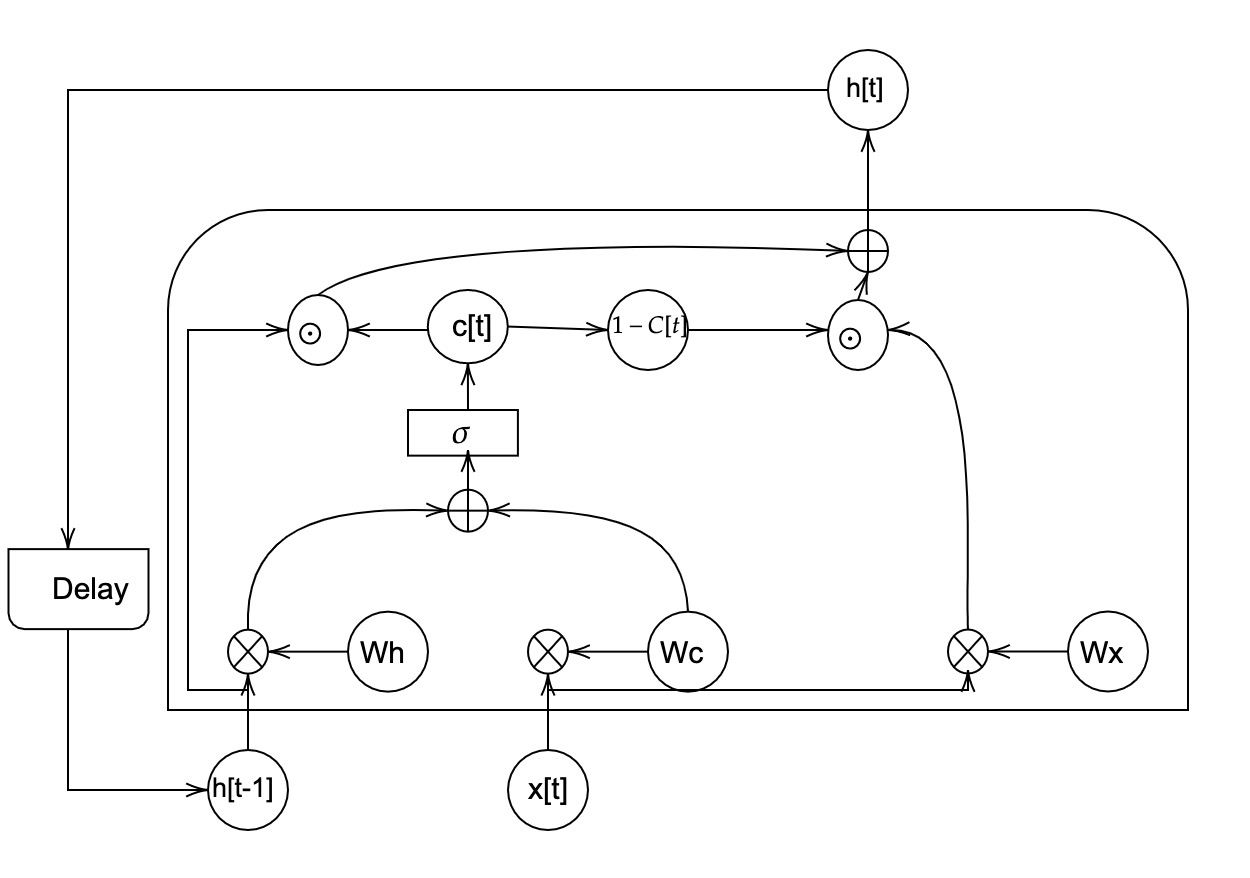
\includegraphics[width=\linewidth]{./images/1-2a.png}




% \tikzset{every picture/.style={line width=0.75pt}} %set default line width to 0.75pt        

% \begin{tikzpicture}[x=0.75pt,y=0.75pt,yscale=-0.5,xscale=0.5]
% %uncomment if require: \path (0,555); %set diagram left start at 0, and has height of 555

% %Shape: Circle [id:dp4165544180946521] 
% \draw   (260,410) .. controls (260,398.95) and (268.95,390) .. (280,390) .. controls (291.05,390) and (300,398.95) .. (300,410) .. controls (300,421.05) and (291.05,430) .. (280,430) .. controls (268.95,430) and (260,421.05) .. (260,410) -- cycle ;
% %Shape: Ellipse [id:dp9223708108057183] 
% \draw   (219.9,178.37) .. controls (219.87,168.25) and (228.8,160.03) .. (239.85,160) .. controls (250.89,159.97) and (259.87,168.15) .. (259.9,178.27) .. controls (259.93,188.39) and (250.99,196.61) .. (239.95,196.64) .. controls (228.9,196.67) and (219.92,188.49) .. (219.9,178.37) -- cycle ;
% %Shape: Circle [id:dp4522347400322082] 
% \draw   (110,410) .. controls (110,398.95) and (118.95,390) .. (130,390) .. controls (141.05,390) and (150,398.95) .. (150,410) .. controls (150,421.05) and (141.05,430) .. (130,430) .. controls (118.95,430) and (110,421.05) .. (110,410) -- cycle ;
% %Straight Lines [id:da9986292572061513] 
% \draw    (130,390) -- (130,353.83) ;
% \draw [shift={(130,351.83)}, rotate = 90] [color={rgb, 255:red, 0; green, 0; blue, 0 }  ][line width=0.75]    (10.93,-3.29) .. controls (6.95,-1.4) and (3.31,-0.3) .. (0,0) .. controls (3.31,0.3) and (6.95,1.4) .. (10.93,3.29)   ;
% %Shape: Circle [id:dp6325062725375508] 
% \draw   (330,340.83) .. controls (330,329.79) and (338.95,320.83) .. (350,320.83) .. controls (361.05,320.83) and (370,329.79) .. (370,340.83) .. controls (370,351.88) and (361.05,360.83) .. (350,360.83) .. controls (338.95,360.83) and (330,351.88) .. (330,340.83) -- cycle ;
% %Flowchart: Summing Junction [id:dp15030926103510023] 
% \draw   (270,340.83) .. controls (270,334.76) and (274.48,329.83) .. (280,329.83) .. controls (285.52,329.83) and (290,334.76) .. (290,340.83) .. controls (290,346.91) and (285.52,351.83) .. (280,351.83) .. controls (274.48,351.83) and (270,346.91) .. (270,340.83) -- cycle ; \draw   (272.93,333.06) -- (287.07,348.61) ; \draw   (287.07,333.06) -- (272.93,348.61) ;
% %Straight Lines [id:da8629901835191436] 
% \draw    (280,390) -- (280,353.83) ;
% \draw [shift={(280,351.83)}, rotate = 90] [color={rgb, 255:red, 0; green, 0; blue, 0 }  ][line width=0.75]    (10.93,-3.29) .. controls (6.95,-1.4) and (3.31,-0.3) .. (0,0) .. controls (3.31,0.3) and (6.95,1.4) .. (10.93,3.29)   ;
% %Straight Lines [id:da6490670874472464] 
% \draw    (330,340.83) -- (292,340.83) ;
% \draw [shift={(290,340.83)}, rotate = 360] [color={rgb, 255:red, 0; green, 0; blue, 0 }  ][line width=0.75]    (10.93,-3.29) .. controls (6.95,-1.4) and (3.31,-0.3) .. (0,0) .. controls (3.31,0.3) and (6.95,1.4) .. (10.93,3.29)   ;
% %Shape: Circle [id:dp2666240029592133] 
% \draw   (180,340.83) .. controls (180,329.79) and (188.95,320.83) .. (200,320.83) .. controls (211.05,320.83) and (220,329.79) .. (220,340.83) .. controls (220,351.88) and (211.05,360.83) .. (200,360.83) .. controls (188.95,360.83) and (180,351.88) .. (180,340.83) -- cycle ;
% %Flowchart: Summing Junction [id:dp8761261711506867] 
% \draw   (120,340.83) .. controls (120,334.76) and (124.48,329.83) .. (130,329.83) .. controls (135.52,329.83) and (140,334.76) .. (140,340.83) .. controls (140,346.91) and (135.52,351.83) .. (130,351.83) .. controls (124.48,351.83) and (120,346.91) .. (120,340.83) -- cycle ; \draw   (122.93,333.06) -- (137.07,348.61) ; \draw   (137.07,333.06) -- (122.93,348.61) ;
% %Straight Lines [id:da679433946453218] 
% \draw    (180,340.83) -- (142,340.83) ;
% \draw [shift={(140,340.83)}, rotate = 360] [color={rgb, 255:red, 0; green, 0; blue, 0 }  ][line width=0.75]    (10.93,-3.29) .. controls (6.95,-1.4) and (3.31,-0.3) .. (0,0) .. controls (3.31,0.3) and (6.95,1.4) .. (10.93,3.29)   ;
% %Flowchart: Or [id:dp2066058485117146] 
% \draw   (230,270.33) .. controls (230,264.54) and (234.48,259.83) .. (240,259.83) .. controls (245.52,259.83) and (250,264.54) .. (250,270.33) .. controls (250,276.13) and (245.52,280.83) .. (240,280.83) .. controls (234.48,280.83) and (230,276.13) .. (230,270.33) -- cycle ; \draw   (230,270.33) -- (250,270.33) ; \draw   (240,259.83) -- (240,280.83) ;
% %Rounded Same Side Corner Rect [id:dp3529851154126782] 
% \draw   (90,170) .. controls (90,142.39) and (112.39,120) .. (140,120) -- (550,120) .. controls (577.61,120) and (600,142.39) .. (600,170) -- (600,370) .. controls (600,370) and (600,370) .. (600,370) -- (90,370) .. controls (90,370) and (90,370) .. (90,370) -- cycle ;
% %Curve Lines [id:da9613936658224065] 
% \draw    (130,329.83) .. controls (127.03,270.43) and (182.87,268.86) .. (228.62,270.29) ;
% \draw [shift={(230,270.33)}, rotate = 181.87] [color={rgb, 255:red, 0; green, 0; blue, 0 }  ][line width=0.75]    (10.93,-3.29) .. controls (6.95,-1.4) and (3.31,-0.3) .. (0,0) .. controls (3.31,0.3) and (6.95,1.4) .. (10.93,3.29)   ;
% %Curve Lines [id:da6191579339823277] 
% \draw    (350,320.83) .. controls (348.01,284.02) and (322.26,268) .. (251.08,270.3) ;
% \draw [shift={(250,270.33)}, rotate = 358.01] [color={rgb, 255:red, 0; green, 0; blue, 0 }  ][line width=0.75]    (10.93,-3.29) .. controls (6.95,-1.4) and (3.31,-0.3) .. (0,0) .. controls (3.31,0.3) and (6.95,1.4) .. (10.93,3.29)   ;
% %Rounded Same Side Corner Rect [id:dp5714915966704466] 
% \draw   (80.25,321.56) .. controls (80.25,325.98) and (76.67,329.56) .. (72.25,329.56) -- (18.25,329.56) .. controls (13.83,329.56) and (10.25,325.98) .. (10.25,321.56) -- (10.25,289.56) .. controls (10.25,289.56) and (10.25,289.56) .. (10.25,289.56) -- (80.25,289.56) .. controls (80.25,289.56) and (80.25,289.56) .. (80.25,289.56) -- cycle ;
% %Straight Lines [id:da910848724599419] 
% \draw    (40,330) -- (40,410) -- (108,410) ;
% \draw [shift={(110,410)}, rotate = 180] [color={rgb, 255:red, 0; green, 0; blue, 0 }  ][line width=0.75]    (10.93,-3.29) .. controls (6.95,-1.4) and (3.31,-0.3) .. (0,0) .. controls (3.31,0.3) and (6.95,1.4) .. (10.93,3.29)   ;
% %Straight Lines [id:da31998338296119666] 
% \draw    (130,360) -- (100,360) -- (100,180) -- (148,180) ;
% \draw [shift={(150,180)}, rotate = 180] [color={rgb, 255:red, 0; green, 0; blue, 0 }  ][line width=0.75]    (10.93,-3.29) .. controls (6.95,-1.4) and (3.31,-0.3) .. (0,0) .. controls (3.31,0.3) and (6.95,1.4) .. (10.93,3.29)   ;
% %Flowchart: Connector [id:dp45942804839114926] 
% \draw   (150,180) .. controls (150,170.34) and (156.72,162.5) .. (165,162.5) .. controls (173.28,162.5) and (180,170.34) .. (180,180) .. controls (180,189.66) and (173.28,197.5) .. (165,197.5) .. controls (156.72,197.5) and (150,189.66) .. (150,180) -- cycle ;
% %Straight Lines [id:da0556335646132291] 
% \draw    (220,180) -- (182,180) ;
% \draw [shift={(180,180)}, rotate = 360] [color={rgb, 255:red, 0; green, 0; blue, 0 }  ][line width=0.75]    (10.93,-3.29) .. controls (6.95,-1.4) and (3.31,-0.3) .. (0,0) .. controls (3.31,0.3) and (6.95,1.4) .. (10.93,3.29)   ;
% %Shape: Circle [id:dp06260340458158553] 
% \draw   (310,180) .. controls (310,168.95) and (318.95,160) .. (330,160) .. controls (341.05,160) and (350,168.95) .. (350,180) .. controls (350,191.05) and (341.05,200) .. (330,200) .. controls (318.95,200) and (310,191.05) .. (310,180) -- cycle ;
% %Straight Lines [id:da44665055556010635] 
% \draw    (259.9,178.27) -- (308,179.93) ;
% \draw [shift={(310,180)}, rotate = 181.98] [color={rgb, 255:red, 0; green, 0; blue, 0 }  ][line width=0.75]    (10.93,-3.29) .. controls (6.95,-1.4) and (3.31,-0.3) .. (0,0) .. controls (3.31,0.3) and (6.95,1.4) .. (10.93,3.29)   ;
% %Shape: Circle [id:dp25947083544071936] 
% \draw   (540,340.75) .. controls (540,329.71) and (548.95,320.75) .. (560,320.75) .. controls (571.05,320.75) and (580,329.71) .. (580,340.75) .. controls (580,351.8) and (571.05,360.75) .. (560,360.75) .. controls (548.95,360.75) and (540,351.8) .. (540,340.75) -- cycle ;
% %Flowchart: Summing Junction [id:dp20738446953351253] 
% \draw   (480,340.75) .. controls (480,334.68) and (484.48,329.75) .. (490,329.75) .. controls (495.52,329.75) and (500,334.68) .. (500,340.75) .. controls (500,346.83) and (495.52,351.75) .. (490,351.75) .. controls (484.48,351.75) and (480,346.83) .. (480,340.75) -- cycle ; \draw   (482.93,332.97) -- (497.07,348.53) ; \draw   (497.07,332.97) -- (482.93,348.53) ;
% %Straight Lines [id:da31023981797684663] 
% \draw    (540,340.75) -- (502,340.75) ;
% \draw [shift={(500,340.75)}, rotate = 360] [color={rgb, 255:red, 0; green, 0; blue, 0 }  ][line width=0.75]    (10.93,-3.29) .. controls (6.95,-1.4) and (3.31,-0.3) .. (0,0) .. controls (3.31,0.3) and (6.95,1.4) .. (10.93,3.29)   ;
% %Curve Lines [id:da6556798059725317] 
% \draw    (490,329.75) .. controls (488.02,293.12) and (499.76,179.31) .. (451.48,179.95) ;
% \draw [shift={(450,180)}, rotate = 356.57] [color={rgb, 255:red, 0; green, 0; blue, 0 }  ][line width=0.75]    (10.93,-3.29) .. controls (6.95,-1.4) and (3.31,-0.3) .. (0,0) .. controls (3.31,0.3) and (6.95,1.4) .. (10.93,3.29)   ;
% %Straight Lines [id:da8635105144898305] 
% \draw    (280,360) -- (490,360) -- (490,352) ;
% \draw [shift={(490,350)}, rotate = 90] [color={rgb, 255:red, 0; green, 0; blue, 0 }  ][line width=0.75]    (10.93,-3.29) .. controls (6.95,-1.4) and (3.31,-0.3) .. (0,0) .. controls (3.31,0.3) and (6.95,1.4) .. (10.93,3.29)   ;
% %Shape: Rectangle [id:dp4511785550674474] 
% \draw   (210,220) -- (264.95,220) -- (264.95,242.82) -- (210,242.82) -- cycle ;
% %Straight Lines [id:da8013495670932107] 
% \draw    (240,259.83) -- (240,242) ;
% \draw [shift={(240,240)}, rotate = 90] [color={rgb, 255:red, 0; green, 0; blue, 0 }  ][line width=0.75]    (10.93,-3.29) .. controls (6.95,-1.4) and (3.31,-0.3) .. (0,0) .. controls (3.31,0.3) and (6.95,1.4) .. (10.93,3.29)   ;
% %Straight Lines [id:da6970814526266598] 
% \draw    (240,220) -- (239.95,198.64) ;
% \draw [shift={(239.95,196.64)}, rotate = 89.87] [color={rgb, 255:red, 0; green, 0; blue, 0 }  ][line width=0.75]    (10.93,-3.29) .. controls (6.95,-1.4) and (3.31,-0.3) .. (0,0) .. controls (3.31,0.3) and (6.95,1.4) .. (10.93,3.29)   ;
% %Flowchart: Or [id:dp20373371776267235] 
% \draw   (430,180) .. controls (430,174.48) and (434.48,170) .. (440,170) .. controls (445.52,170) and (450,174.48) .. (450,180) .. controls (450,185.52) and (445.52,190) .. (440,190) .. controls (434.48,190) and (430,185.52) .. (430,180) -- cycle ; \draw   (430,180) -- (450,180) ; \draw   (440,170) -- (440,190) ;
% %Straight Lines [id:da14993543932793973] 
% \draw    (350,180) -- (428,180) ;
% \draw [shift={(430,180)}, rotate = 180] [color={rgb, 255:red, 0; green, 0; blue, 0 }  ][line width=0.75]    (10.93,-3.29) .. controls (6.95,-1.4) and (3.31,-0.3) .. (0,0) .. controls (3.31,0.3) and (6.95,1.4) .. (10.93,3.29)   ;
% %Straight Lines [id:da9604810362940497] 
% \draw    (440,170) -- (440,82) ;
% \draw [shift={(440,80)}, rotate = 90] [color={rgb, 255:red, 0; green, 0; blue, 0 }  ][line width=0.75]    (10.93,-3.29) .. controls (6.95,-1.4) and (3.31,-0.3) .. (0,0) .. controls (3.31,0.3) and (6.95,1.4) .. (10.93,3.29)   ;
% %Shape: Circle [id:dp582477125625587] 
% \draw   (420,60) .. controls (420,48.95) and (428.95,40) .. (440,40) .. controls (451.05,40) and (460,48.95) .. (460,60) .. controls (460,71.05) and (451.05,80) .. (440,80) .. controls (428.95,80) and (420,71.05) .. (420,60) -- cycle ;
% %Straight Lines [id:da08248143917192818] 
% \draw    (420,60) -- (40,60) -- (40,288) ;
% \draw [shift={(40,290)}, rotate = 270] [color={rgb, 255:red, 0; green, 0; blue, 0 }  ][line width=0.75]    (10.93,-3.29) .. controls (6.95,-1.4) and (3.31,-0.3) .. (0,0) .. controls (3.31,0.3) and (6.95,1.4) .. (10.93,3.29)   ;

% % Text Node
% \draw (149,169) node [anchor=north west][inner sep=0.75pt]    {$\odot $};
% % Text Node
% \draw (267,398) node [anchor=north west][inner sep=0.75pt]   [align=left] {x[t]};
% % Text Node
% \draw (228.87,166.39) node [anchor=north west][inner sep=0.75pt]  [rotate=-359.85] [align=left] {c[t]};
% % Text Node
% \draw (109,397) node [anchor=north west][inner sep=0.75pt]   [align=left] {{\small h[t-1]}};
% % Text Node
% \draw (333,329.83) node [anchor=north west][inner sep=0.75pt]   [align=left] {Wc};
% % Text Node
% \draw (183,329.83) node [anchor=north west][inner sep=0.75pt]   [align=left] {Wh};
% % Text Node
% \draw (29,298) node [anchor=north west][inner sep=0.75pt]   [align=left] {Delay};
% % Text Node
% \draw (309,169) node [anchor=north west][inner sep=0.75pt]  [font=\scriptsize]  {$1-C[ t]$};
% % Text Node
% \draw (543,329.75) node [anchor=north west][inner sep=0.75pt]   [align=left] {Wx};
% % Text Node
% \draw (229,219) node [anchor=north west][inner sep=0.75pt]    {$\sigma $};
% % Text Node
% \draw (426,47) node [anchor=north west][inner sep=0.75pt]   [align=left] {{\small h[t]}};
% \end{tikzpicture}

\subsubsection*{(b)}
where $\sigma$ is element-wise sigmoid, $x[t] \in \mathbb{R}^n$, $h[t] \in \mathbb{R}^m$, $W_c \in \mathbb{R}^{m \times n}$,  $W_h \in \mathbb{R}^{m \times m}$, $W_x \in \mathbb{R}^{m \times n}$, $\odot$ is Hadamard product, $h[0] \doteq 0$.

\begin{align}
    C[t] &= \sigma(W_c x[t] + W_h  h[t-1] ) 
\end{align}

\begin{align}
    C[t] &\in (\mathbb{R}^{(m \times n)(n)} +\mathbb{R}^{(m \times m)(m)})\\
    &\in \mathbb{R}^{m}
\end{align}

\subsubsection*{(c)}
(10 pts) Suppose that we run the RNN to get a sequence of $h[t]$ for t from 1 to $K$. Assuming we know the derivative $\frac{\partial \ell}{\partial h[t]}$, provide dimension of and an expression for values of $\frac{\partial \ell}{\partial W_x}$. What are the similarities of backward pass and forward pass in this RNN?

\begin{align}
    \frac{\partial \ell}{\partial W_x} \in \mathcal{R}^{m \times n} \\
    \frac{\partial \ell}{\partial h[t]} \in \mathcal{R}^{m \times 1} 
\end{align}

\begin{align}
    h[t] = c[t] \odot h[{t-1}] + (1-c[t]) \odot W_x x[t]
\end{align}

\begin{align}
    \frac{\partial \ell}{\partial W_x} &= \frac{\partial \ell}{\partial h[t]}  \frac{\partial h[t]}{\partial W_x} \\
    &= (1-c[t]) \odot (\frac{\partial \ell}{\partial h[t]}) x[t]^T
\end{align}

The similarities are that the forward pass is a function of the current input $x[t]$ and the previous hidden state $h[t-1]$, and the backward pass is a function of the current hidden state $h[t]$ and the next input $x[t]$.

\subsubsection*{(d)}

\begin{align}
    \frac{\partial \ell}{\partial h[t-1]} &= \frac{\partial \ell}{\partial h[t]}  
    (\frac{\partial h[t]}{\partial h[t-1]} + \frac{\partial h[t]}{\partial c[t]}  \frac{\partial c[t]}{\partial h[t-1]})
\end{align}

There is a path from h[t] to h[t-1] without passing through the sigmoid, which can somehow prevent the gradient vanishing problem.

But for the gradient exploding, there is no gate to regularize the gradient, there is a direct path from h[t] to h[t-1], if the gradient is too large, it will make all the steps gradients explode, the model will still suffer from the gradient exploding problem.


\subsection{Debugging loss curves (10pts)}
\label{debug_loss}

In the class on Wednesday, February 16, when working with notebook \\
\texttt{08-seq\_classification}, we saw RNN training curves. In Section 8 ``Visualize LSTM'', we observed some ``kinks'' in the loss curve.

\begin{center}
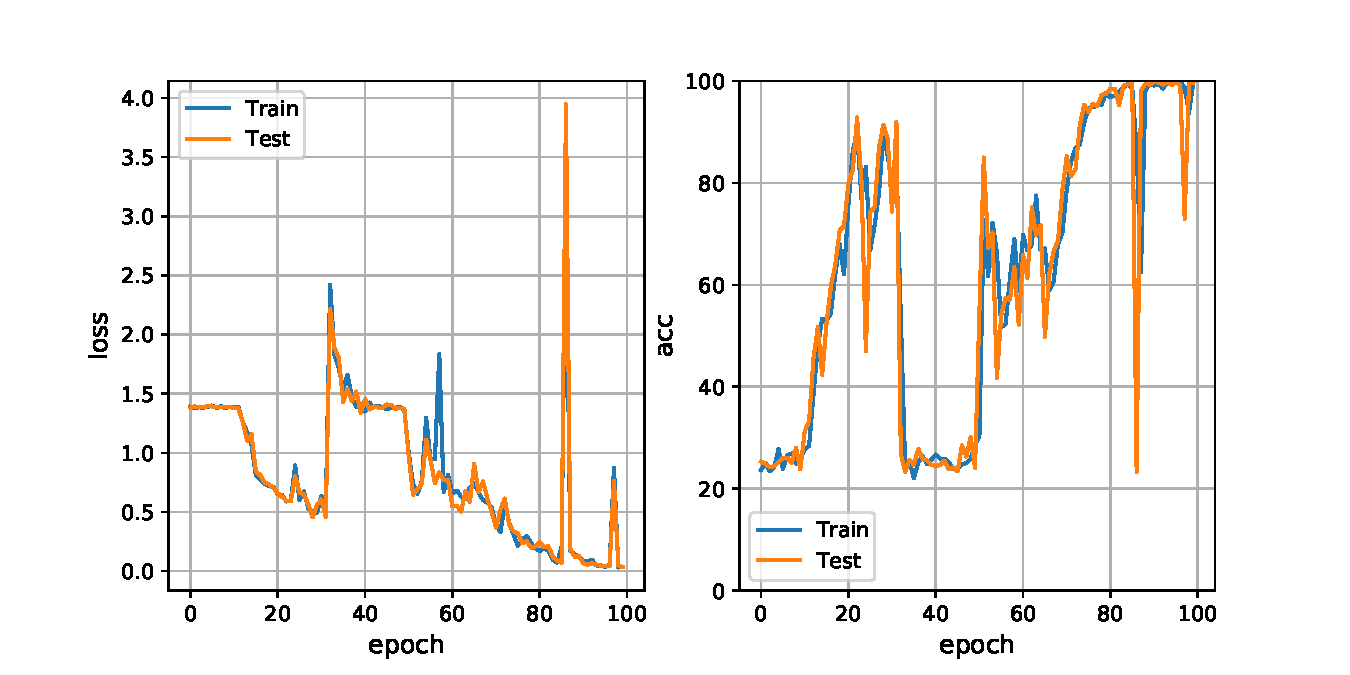
\includegraphics[scale=0.5]{plots.pdf}
\end{center}

\begin{enumerate}
    \item (2pts) What caused the spikes on the left?
    \item (2pts) How can they be higher than the initial value of the loss?
    \item (3pts) What are some ways to fix them?
    \item (3pts) Explain why the loss and accuracy are at these values before training starts. You may need to check the task definition in the notebook.
\end{enumerate}

\textbf{Solution:}
\subsubsection*{1}
The network get very large gradients in the wrong direction.

\subsubsection*{2}
The wrong gradients step is very large, which is larger than the cummulative gradient step from the training start.
\subsubsection*{3}
Clipping the gradients to prevent large wrong gradients. Momentum can also help.

\subsubsection*{4}
% The MODERATE difficulty task definition is 
There are 4 sequence classes Q, R, S, U, thus the initial acc is 0.25 due to random guessing.

The loss is at the initial value before training starts.

For Cross Entory, the loss is is the expectation of the uniform distribution and the one hot distributino.

\begin{align}
    Loss  =  - 1 * log(1/4)
          =  log(4)
          =  1.3863 \\ \text{(e as the base)}
\end{align}
